%==============================================================================
% MAT3300 Mathematical Modeling — Final Project Report Template (single file)
% Problem C: 2021 ICM Problem D — The Influence of Music
%
% Structure per Final_Project_Guidelines.pdf and the Problem C statement:
%   1. One-page Summary Sheet  (team members' full names + student IDs at the
%      top, as required by the course guidelines)
%   2. Table of Contents
%   3. Complete solution (main body)
%   4. One-page document to the ICM Society  (value of approach, effect of
%      richer data, further study recommendations — required by Problem C)
%   5. References
%   6. Contribution statement  (EXTRA page, NOT counted in the 25-page limit)
%
% TOTAL page budget for items 1–5: at most 25 pages.
%
% Compile:  pdflatex main.tex  (run TWICE so the ToC and cross-references
%           resolve), or: latexmk -pdf main.tex
%==============================================================================
\documentclass[11pt,letterpaper]{article}

%------------------------------------------------------------------------------
% Page layout & typography
%------------------------------------------------------------------------------
\usepackage[margin=1in]{geometry}
\usepackage{microtype}
\usepackage{fancyhdr}
\usepackage{titlesec}
\usepackage{setspace}

%------------------------------------------------------------------------------
% Math
%------------------------------------------------------------------------------
\usepackage{amsmath,amssymb,amsfonts,amsthm}
\usepackage{mathtools}
\usepackage{bm}
\usepackage{siunitx}

%------------------------------------------------------------------------------
% Graphics, tables, figures
%------------------------------------------------------------------------------
\usepackage{graphicx}
\graphicspath{{./figures/}}     % put all figure files in ./figures/
\usepackage{booktabs}
\usepackage{multirow}
\usepackage{longtable}
\usepackage{tabularx}
\usepackage{threeparttable}
\usepackage{caption}
\usepackage{subcaption}
\captionsetup{font=small,labelfont=bf}

%------------------------------------------------------------------------------
% Algorithms, code listings, colors
%------------------------------------------------------------------------------
\usepackage{algorithm}
\usepackage{algpseudocode}
\usepackage{listings}
\usepackage{xcolor}
\lstset{
  language=Python, basicstyle=\ttfamily\footnotesize,
  keywordstyle=\color{blue!60!black}\bfseries,
  backgroundcolor=\color{gray!6}, frame=single, breaklines=true,
  numbers=left, numberstyle=\tiny\color{gray}
}

%------------------------------------------------------------------------------
% Diagrams (optional)
%------------------------------------------------------------------------------
\usepackage{tikz}
\usetikzlibrary{arrows.meta,positioning,shapes.geometric}

%------------------------------------------------------------------------------
% Lists, cross-references, hyperlinks (hyperref LAST, cleveref after it)
%------------------------------------------------------------------------------
\usepackage{enumitem}
\usepackage[colorlinks=true,linkcolor=blue,citecolor=blue,urlcolor=blue]{hyperref}
\usepackage{cleveref}

\numberwithin{equation}{section}

%------------------------------------------------------------------------------
% Header / footer
%------------------------------------------------------------------------------
\pagestyle{fancy}
\fancyhf{}
\fancyhead[L]{\small MAT3300 Final Project}
\fancyfoot[C]{\thepage}
\renewcommand{\headrulewidth}{0.4pt}

%==============================================================================
% Team information
%==============================================================================
\newcommand{\TeamMembers}{%
  Yu Zihan (123090773)\quad
  Qian Chenghao (123090452)\quad
  Li Peixuan (123090276)}

%==============================================================================
\begin{document}
%==============================================================================

%------------------------------------------------------------------------------
% 1. SUMMARY SHEET — one page, must stand on its own; write it LAST.
%    Cover: problem, approach, key results (with numbers), validation, conclusion.
%------------------------------------------------------------------------------
\thispagestyle{empty}
\begin{center}
  {\LARGE\bfseries Measuring Musical Influence: A Directed-Network Approach
   to the Evolution of Music}\\[10pt]
  {\normalsize \TeamMembers}\\[4pt]
  {\small MAT3300 Mathematical Modeling --- Final Project, CUHK-Shenzhen}
\end{center}
\vspace{0.8em}
\noindent\rule{\textwidth}{0.6pt}
\vspace{0.8em}
\begin{center}
  {\Large\bfseries Summary}
\end{center}
% TODO: summary text (problem -> approach -> key results -> validation -> conclusion)
\vspace{0.6em}
\noindent\textbf{Keywords:} directed network; musical influence; similarity
measurement; genre evolution; PageRank; sensitivity analysis
\newpage

%------------------------------------------------------------------------------
% 2. TABLE OF CONTENTS
%------------------------------------------------------------------------------
\tableofcontents
\newpage

%------------------------------------------------------------------------------
% 3. COMPLETE SOLUTION
%------------------------------------------------------------------------------
\pagenumbering{arabic}

\section{Introduction and Problem Restatement}\label{sec:intro}
% TODO: background; restatement of the 7 tasks from Problem C; roadmap.

\section{Assumptions and Justifications}\label{sec:assumptions}

\begin{enumerate}[label=\textbf{A\arabic*.},leftmargin=2.2em]
  \item \label{assump:weight}
  \textbf{Edge existence, not strength.} Each record in the influence data
  states that one artist reported another as an influence; it carries no
  information about \emph{how strong} that influence was. In Model~I we
  therefore assign every reported pair a uniform weight \(w_{ij}=1\). Any
  strength information must be constructed from other evidence; we do so in
  Model~II, where feature-based quantities are attached to edges.
  \item \label{assump:decade}
  \textbf{Active-start decade is an artist attribute.} The field
  \texttt{active\_start} is recorded at decade granularity and describes when
  an artist \emph{began} performing. It is not the date at which any
  particular influence occurred, and influence may act years after the
  follower's debut. We therefore use decades only for grouping (cohorts,
  era comparisons) and make no causal timing claims from them.
  \item \label{assump:reverse}
  \textbf{Time-order reversals are record noise.} A small fraction of edges
  (733 of 42{,}770, 1.7\%) connect an influencer whose active-start decade is
  \emph{later} than the follower's. Because decades are coarse and
  same-generation artists routinely credit each other, we interpret these as
  record imprecision or mutual influence rather than impossible relations,
  and retain them in the primary network; \cref{subsec:q1-robustness}
  quantifies their effect.
  \item \label{assump:genre}
  \textbf{One main genre per artist.} Each artist carries a single
  \texttt{main\_genre} label (AllMusic macro-genres). The label is coarse ---
  e.g.\ ``Pop/Rock'' spans many sub-styles --- so all genre-level statements
  refer to these macro-categories, and we revisit the labelling granularity
  when interpreting genre-based results.
\end{enumerate}

\section{Notation}\label{sec:notation}

\Cref{tab:notation} lists the symbols used throughout the report.

\begin{table}[htbp]
\centering
\caption{Main notation.}
\label{tab:notation}
\begin{tabular}{ll}
\toprule
Symbol & Meaning \\
\midrule
\(G=(V,E)\) & directed influence network; \(i\to j\) means ``\(i\) reported as an influence on \(j\)'' \\
\(N=|V|\)   & number of artists (nodes) \\
\(A_{ij}\)  & adjacency indicator, \(A_{ij}=\mathbf{1}[i\to j\in E]\) \\
\(w_{ij}\)  & edge weight (\(w_{ij}=1\) in Model~I) \\
\(d_i^{\text{out}},\,d_i^{\text{in}}\) & out-/in-degree of node \(i\) \\
\(d_j^{\leftarrow,\text{out}}\) & out-degree of \(j\) within the reversed graph \(G^{\leftarrow}\) \\
\(K_i\)     & outgoing Katz centrality of artist \(i\) \\
\(\alpha\)  & Katz attenuation factor \\
\(\rho\)    & spectral radius of the adjacency matrix \(A\) \\
\(\mathrm{PR}^{\text{rev}}_i\) & reverse PageRank of artist \(i\) (computed on \(G^{\leftarrow}\)) \\
\(\delta\)  & PageRank damping factor (\(\delta=0.85\)) \\
\(C_d\)     & cohort of followers whose active-start decade is \(d\) \\
\(G_S\)     & genre-induced subnetwork over artists of genre \(S\) \\
\(s_{ij}\)  & feature-based similarity between artists \(i\) and \(j\) (Model~II) \\
\(\tilde{\mathbf{x}}_i\) & \(z\)-scored Spotify feature vector of artist \(i\) \\
\(\mathbf{c}_g\), \(\mathbf{c}_g(t)\) & Katz-weighted genre centroid (static / by active-start decade) \\
\(d_{gh}\), \(s_{gh}\) & Euclidean distance / similarity between genre centroids \\
\(F(t),\,P,\,Q\) & genre flow / export / source profiles (Model~III; follower-start decade \(t\)) \\
\(c_{\mathrm{cross}}(t),\,c_K(t)\) & cross-genre edge share; Katz-weighted cross-genre share \\
\(\mathbf{x}(t),\,E(t)\) & yearly \(z\)-feature state; sonic leap \(\|\mathbf{x}(t)-\mathbf{x}(t-1)\|_2\) \\
\(N(t)\) & network restructuring score from \(\Delta c_{\mathrm{cross}}\), \(\Delta c_K\), Katz-mass turnover \\
\bottomrule
\end{tabular}
\end{table}

\section{Data Preprocessing and Exploration}\label{sec:data}

\subsection{The Four Provided Files}\label{subsec:data-files}

The problem provides four files.
\texttt{influence\_data.csv} (42{,}770 rows $\times$ 8 columns) lists
reporter--influence pairs: for each edge it gives both artists' identifiers,
names, main genre and active-start decade. \texttt{full\_music\_data.csv}
(98{,}340 tracks) contains per-track Spotify audio features together with a
stringified list of performing-artist identifiers (4{,}410 tracks involve
more than one artist). \texttt{data\_by\_artist.csv} and
\texttt{data\_by\_year.csv} are Spotify-provided aggregates over 5{,}810
artists and over the years 1921--2020, respectively. Model~I uses only the
influence file; Models~II and~III additionally use the track-level features,
whose preprocessing (multi-artist attribution, count-weighted aggregation,
per-year normalisation) is described there.

\subsection{Cleaning of the Influence Data}\label{subsec:data-cleaning}

The raw influence file requires four repairs before it can be used.
(i)~\emph{Identifier hygiene}: trailing whitespace in artist identifiers and
names is trimmed. (ii)~\emph{Encoding artefacts}: mojibake in some artist
names is repaired by re-decoding the affected strings. (iii)~\emph{Label
repair}: genre labels contain an HTML-escape residue (e.g.\ ``R\&B;''
$\to$ ``R\&B''), which we strip. (iv)~\emph{Type coercion}: active-start
fields are cast to decade integers. After these repairs we check for
duplicated directed pairs; none exist, so all 42{,}770 unique directed pairs
are retained, spanning \(N=5{,}603\) artists.

\subsection{Data-Quality Audit}\label{subsec:data-audit}

Two structural facts of the influence data shape every later model, so we
audit them here rather than inside any single model.

\emph{Time-order consistency.} Decade information allows a consistency
check that the raw data never advertises: in 733 edges (1.7\%) the follower's
active-start decade precedes the influencer's, and in 8{,}477 edges the two
decades coincide. Per Assumption~A3 the 733 reversals are retained in the
primary network and their effect is quantified in
\cref{subsec:q1-robustness}; same-decade edges are kept as same-generation
mutual influence.

\emph{Skewed connectivity and genre concentration.} The out-degree
distribution is heavily right-skewed (mean 11.3, median 5, maximum 615 for
The Beatles), while in-degrees are moderate (median 7, maximum 47): being
cited is bounded by list length, citing is not. Genre labels concentrate
sharply --- Pop/Rock accounts for 56\% of all edges --- and 76.6\% of edges
connect same-genre artists. These facts motivate the log-scale treatment of
degree in \cref{subsec:q1-global}, the cohort view of
\cref{subsec:q1-cohorts}, and the genre-comparison design of Model~III.

\section{Model I: Directed Influence Network}\label{sec:model-influence}

This section addresses Task~1: we build the reported musical-influence network,
develop parameters that capture influence, and describe the resulting structure
both globally and through two complementary lenses (temporal cohorts and a
genre-induced subnetwork).

\subsection{Network Construction}\label{subsec:net-construction}

Using the cleaned edge table of \cref{subsec:data-cleaning}, we model the
influence system as a directed graph \(G=(V,E)\), where each node
\(v\in V\) is an artist (\(|V|=5{,}603\)) and each edge \(i\to j\in E\)
records that the data report artist \(i\) as an influence on artist \(j\)
(\(|E|=42{,}770\)). Because the data record the \emph{existence} of a
reported relation rather than its strength, we assign every edge the
baseline weight \(w_{ij}=1\) (Assumption~A1); constructing edge strengths
from musical evidence is deferred to Model~II. Genre and active-start
decade are attached to nodes as descriptive attributes (Assumption~A2),
and the 733 time-order-reversed edges identified in the data audit are
retained in the primary network (Assumption~A3), with their effect
quantified separately in \cref{subsec:q1-robustness}.

\subsection{Influence Measures and Network Topology}\label{subsec:q1-measures}

We report three measures with deliberately distinct interpretations rather
than a single weighted composite: each answers a different question, and their
agreement (or disagreement) is itself informative.

\paragraph{Out-degree.}
The number of artists who directly name \(i\) as an influence,
\begin{equation}
d_i^{\text{out}}=\sum_{j} A_{ij}, \qquad A_{ij}=\mathbf{1}[i\to j\in E],
\end{equation}
measures \emph{direct} reach. It is transparent but blind to indirect
transmission.

\paragraph{Outgoing Katz centrality (primary measure).}
To capture multi-step influence we use Katz centrality computed on outgoing
paths,
\begin{equation}\label{eq:katz}
K_i=\Bigl[(I-\alpha A)^{-1}\mathbf{1}\Bigr]_i
   =1+\alpha (A\mathbf{1})_i+\alpha^2(A^2\mathbf{1})_i+\cdots,
\end{equation}
which counts all directed walks leaving \(i\), each additional hop discounted
by the attenuation factor \(\alpha\in(0,1/\rho)\), where \(\rho\) is the
spectral radius of \(A\). For our network \(\rho=3.614\), so
\(\alpha<0.2767\) guarantees convergence; we use \(\alpha=0.10\), which keeps
a comfortable margin from the bound while weighting second- and third-step
transmission substantially (a path of length \(\ell\) contributes
\(\alpha^{\ell-1}\)). Intuitively, \(K_i\) rewards artists whose followers
themselves went on to influence many others: influencing one future
``hub'' can be worth more than influencing many dead-end artists.

\paragraph{Reverse PageRank (comparison measure).}
PageRank scores a node by the PageRank of the nodes that point to it. On the
raw edge direction, that would measure \emph{receiving} influence. We therefore
compute PageRank on the reversed graph \(G^{\leftarrow}\), in which every edge
is flipped so that a follower endorses its influencer:
\begin{equation}\label{eq:rpr}
\mathrm{PR}^{\text{rev}}_i=\frac{1-\delta}{N}
 +\delta\sum_{j\to i\,\in\,G^{\leftarrow}}\frac{\mathrm{PR}^{\text{rev}}_j}{d_j^{\leftarrow,\text{out}}},
 \qquad \delta=0.85,
\end{equation}
where \(d_j^{\leftarrow,\text{out}}\) is \(j\)'s out-degree within the
reversed graph (equivalently, its in-degree in \(G\)), so that recognition
flows from reported followers back to the artists they credit. We state
this reversal explicitly because it is the difference between
``being shaped by important artists'' and ``shaping important artists''.

We do \emph{not} merge the three measures into an ad hoc weighted index:
they encode different semantics, and any fixed weighting would be
arbitrary; instead we compare their rankings, and
\cref{subsec:q1-robustness} shows the conclusions are robust to this
choice.

\Cref{tab:q1-topology} summarises the network. The graph is almost fully
connected in the weak sense (99.9\% of artists lie in one weak component),
but fragmented into many strong components: influence, as reported, flows
through a giant downstream cascade rather than forming tightly reciprocated
clusters. The 1{,}829 artists with zero out-degree have no recorded
followers in this dataset---a statement about the data, not proof of
absence of influence; the decade lag between influencer and follower is
consistent with the one-to-two-generation transmission delay expected of
influence.

\begin{table}[htbp]
\centering
\caption{Topology of the reported influence network.}
\label{tab:q1-topology}
\begin{tabular}{lr}
\toprule
Statistic & Value \\
\midrule
Reported pairs (unique directed edges) & 42{,}770 \\
Artists (nodes) & 5{,}603 \\
Weakly connected components & 3 \\
Largest weak component & 5{,}599 (99.9\%) \\
Strongly connected components & 4{,}747 \\
Largest strong component & 778 \\
Artists with zero out-degree & 1{,}829 \\
Artists with zero in-degree & 557 \\
Edges with reversed decade order (retained) & 733 (1.7\%) \\
Edges with same-decade endpoints & 8{,}477 \\
\bottomrule
\end{tabular}
\end{table}

\subsection{Global Results: Leading Influencers}\label{subsec:q1-global}

\Cref{fig:q1-global} presents the primary results. The Katz ranking is led by
Chuck Berry, followed by The Beatles, Muddy Waters, Louis Jordan and Bob
Dylan (\cref{tab:q1-top10}). The contrast between the two panels of
\cref{fig:q1-global} is the central empirical finding of this section:
\emph{direct} and \emph{multi-step} influence agree in bulk
(Spearman \(\rho=0.953\) overall) yet diverge sharply at the top. The Beatles
hold by far the largest direct following (out-degree 615), but Chuck Berry---
with only 159 direct followers---outranks them in Katz terms because his
followers include artists who themselves became massive transmission hubs.
Multi-step credit, in other words, rewards artists whose influence
\emph{propagates} through the network, not merely those who accumulate the
most direct citations. Muddy Waters, Louis Jordan, Hank Williams and Howlin'
Wolf illustrate the same mechanism from older generations: modest direct
lists, but followers who carried blues and jazz idioms into the rock era.

\begin{table}[htbp]
\centering
\caption{Top-10 artists by outgoing Katz centrality (\(\alpha=0.10\)),
with direct out-degree and rank under reverse PageRank for comparison.}
\label{tab:q1-top10}
\begin{tabular}{rlrrr}
\toprule
Rank & Artist & \(K_i\) & \(d_i^{\text{out}}\) & PR\(^{\text{rev}}\) rank \\
\midrule
1 & Chuck Berry      & 713.4 & 159 & 19 \\
2 & The Beatles      & 691.8 & 615 & 7  \\
3 & Muddy Waters     & 580.0 & 113 & 13 \\
4 & Louis Jordan     & 549.5 & 53  & 4  \\
5 & Bob Dylan        & 545.3 & 389 & 14 \\
6 & Hank Williams    & 543.6 & 184 & 18 \\
7 & Little Richard   & 537.6 & 88  & 26 \\
8 & Elvis Presley    & 515.2 & 166 & 27 \\
9 & Roy Brown        & 513.2 & 34  & 25 \\
10 & Howlin' Wolf    & 435.9 & 99  & 29 \\
\bottomrule
\end{tabular}
\end{table}

\begin{figure}[htbp]
\centering
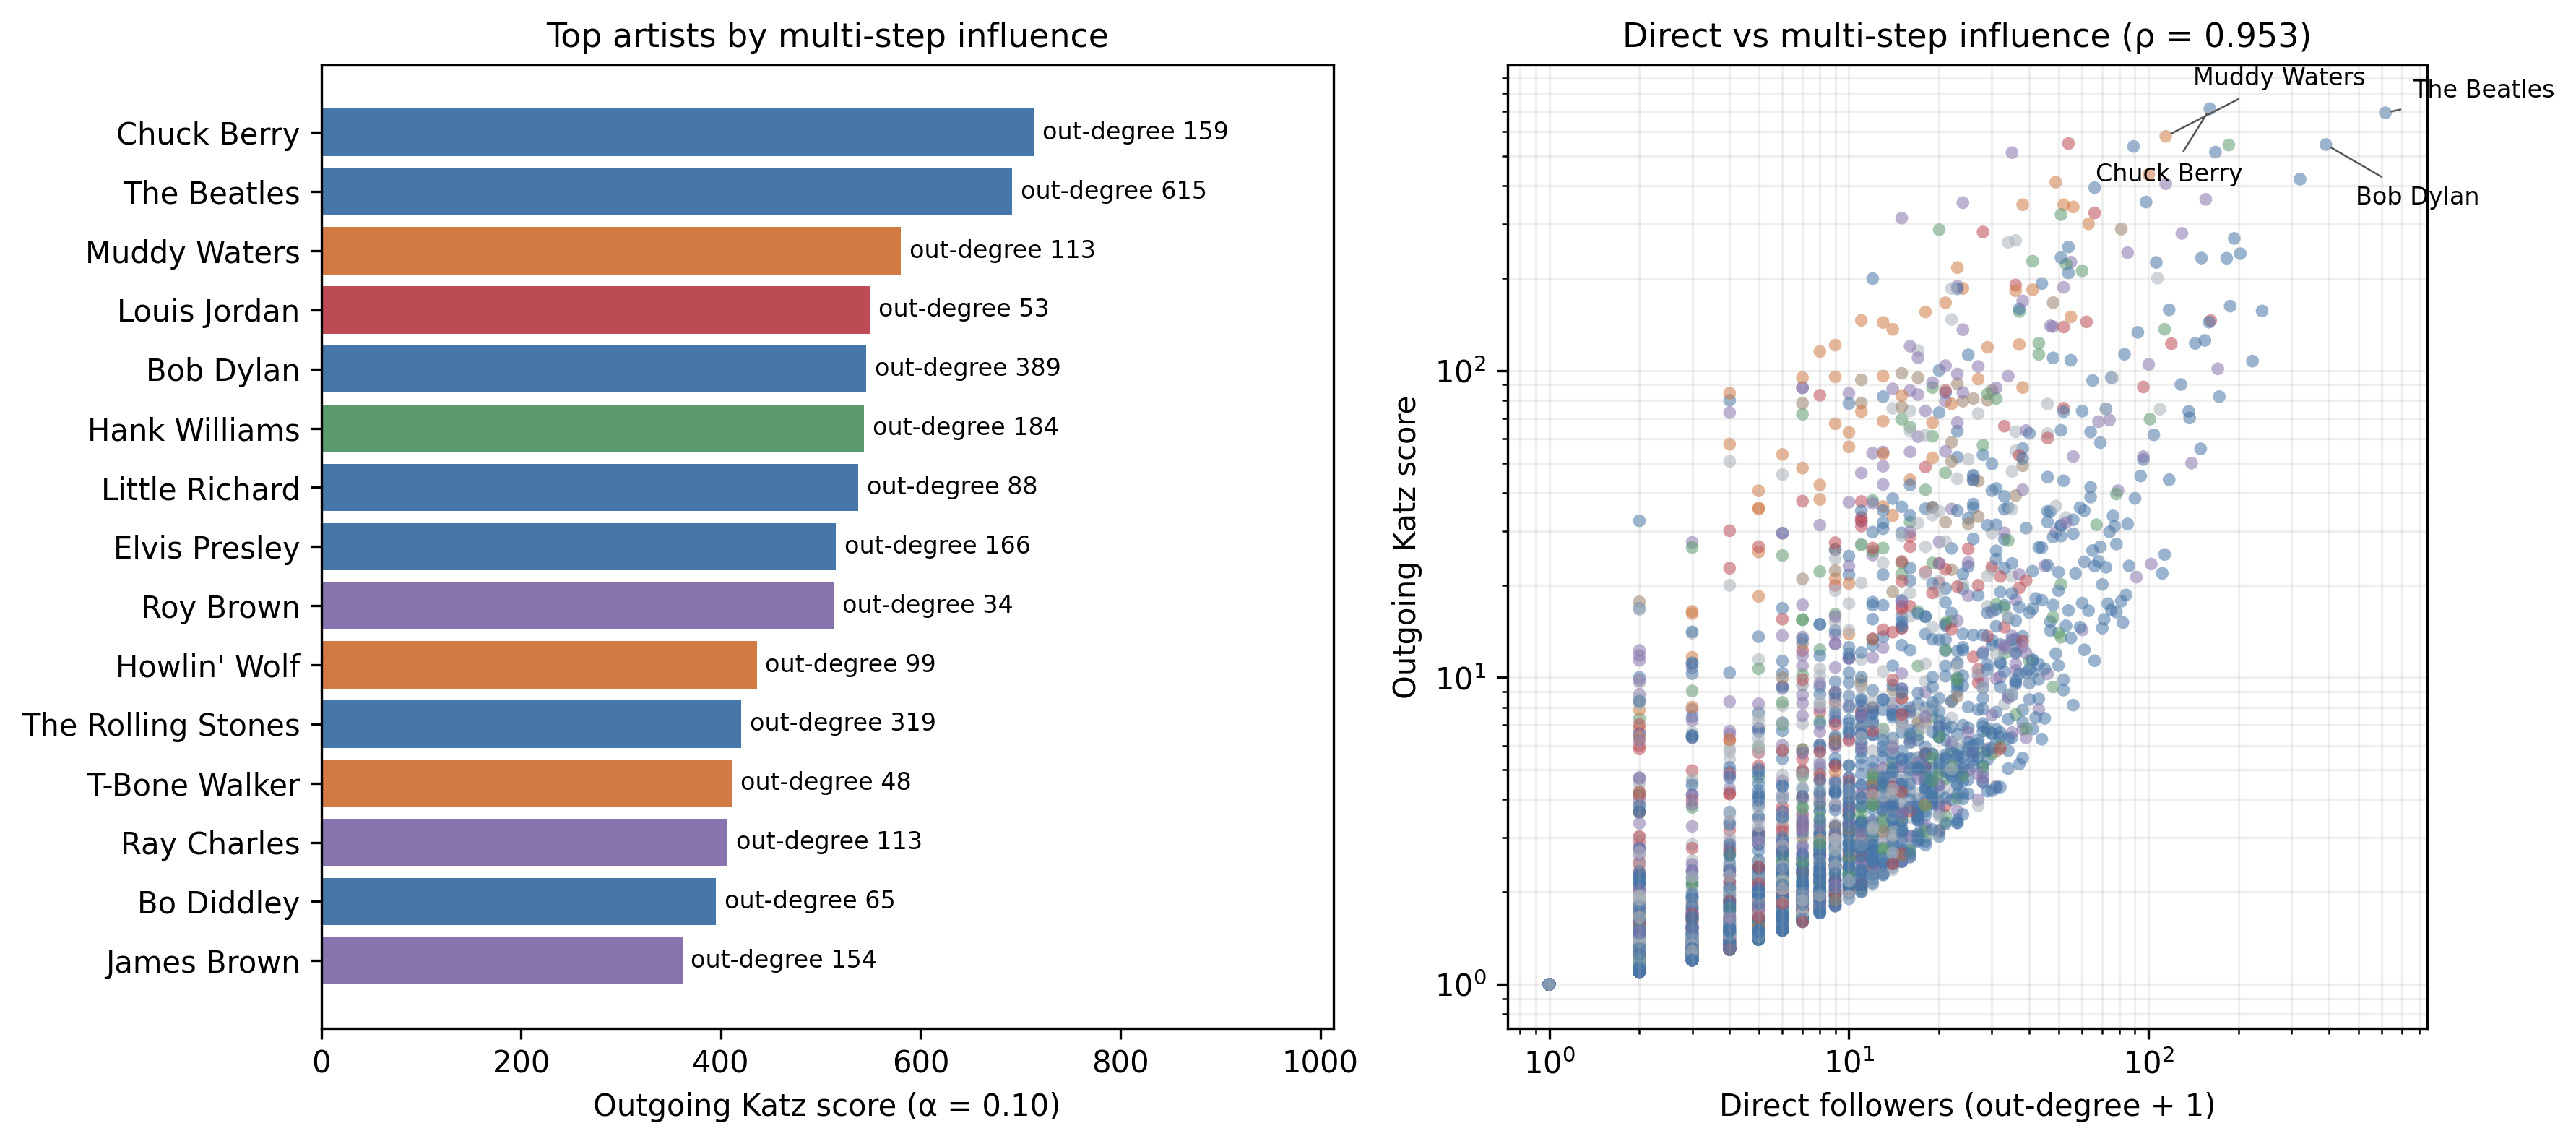
\includegraphics[width=\textwidth]{fig1_global_influence.png}
\caption{Global influence rankings. \emph{Left:} top-15 artists by outgoing
Katz score (\(\alpha=0.10\)); bar colour encodes the artist's main genre and
the annotation gives the raw out-degree. \emph{Right:} direct followers
(out-degree) versus Katz score on log--log axes; artists far above the
diagonal owe their position to indirect, multi-step transmission
(Spearman \(\rho=0.953\)).}
\label{fig:q1-global}
\end{figure}

The reverse-PageRank column of \cref{tab:q1-top10} reveals a systematic
difference in character: its global top ranks are occupied by early-era
artists (Cab Calloway, Billie Holiday and Lester Young lead the overall
ranking), because under recursive endorsement an artist active in the
1930s has had nine decades to accumulate credit. This is the well-known
age bias of centrality measures on growing networks: reverse PageRank
measures \emph{accumulated recognition}, while outgoing Katz measures
\emph{transmission capacity}. We report both and treat the divergence as
informative rather than averaging it away; an era-normalised variant is
discussed as a refinement in \cref{sec:validation}.

\subsection{A Dynamic View: Follower-Start-Decade Cohorts}\label{subsec:q1-cohorts}

To expose the temporal structure of reported influence without claiming exact
influence dates (Assumption~A2), we group all edges by the follower's
active-start decade and recompute the network and Katz scores within each
\emph{follower-start-decade cohort} \(C_d\). A cohort answers the question
``which influencers are credited by the artists who \emph{began} in decade
\(d\)?''---it does not date when the influence happened.

\Cref{fig:q1-cohorts} tracks the 15 artists who most often rank in a cohort's
top 10, and \cref{tab:q1-cohorts} lists cohort sizes and leading names. Three
patterns emerge. First, \emph{generational succession}: swing-era figures
dominate the 1930s--1940s cohorts, the 1950s cohort pivots to country and
early rock, and rock artists take over from the 1960s onward. Second,
\emph{cross-generational persistence}: The Beatles rank inside the top two
of five consecutive cohorts (1960s--2000s), and Bob Dylan never leaves the
top 10 from the 1960s cohort onward. Third, \emph{cohort-specific
arrivals}: Nirvana appears only from the 1990s cohort (rank~1) and David
Bowie peaks in the 1970s--1980s---each cohort reports the canon available
to it. The 2010s cohort is much smaller (811 edges) and its top-10
membership should be read with this sample-size caveat.

\begin{figure}[htbp]
\centering
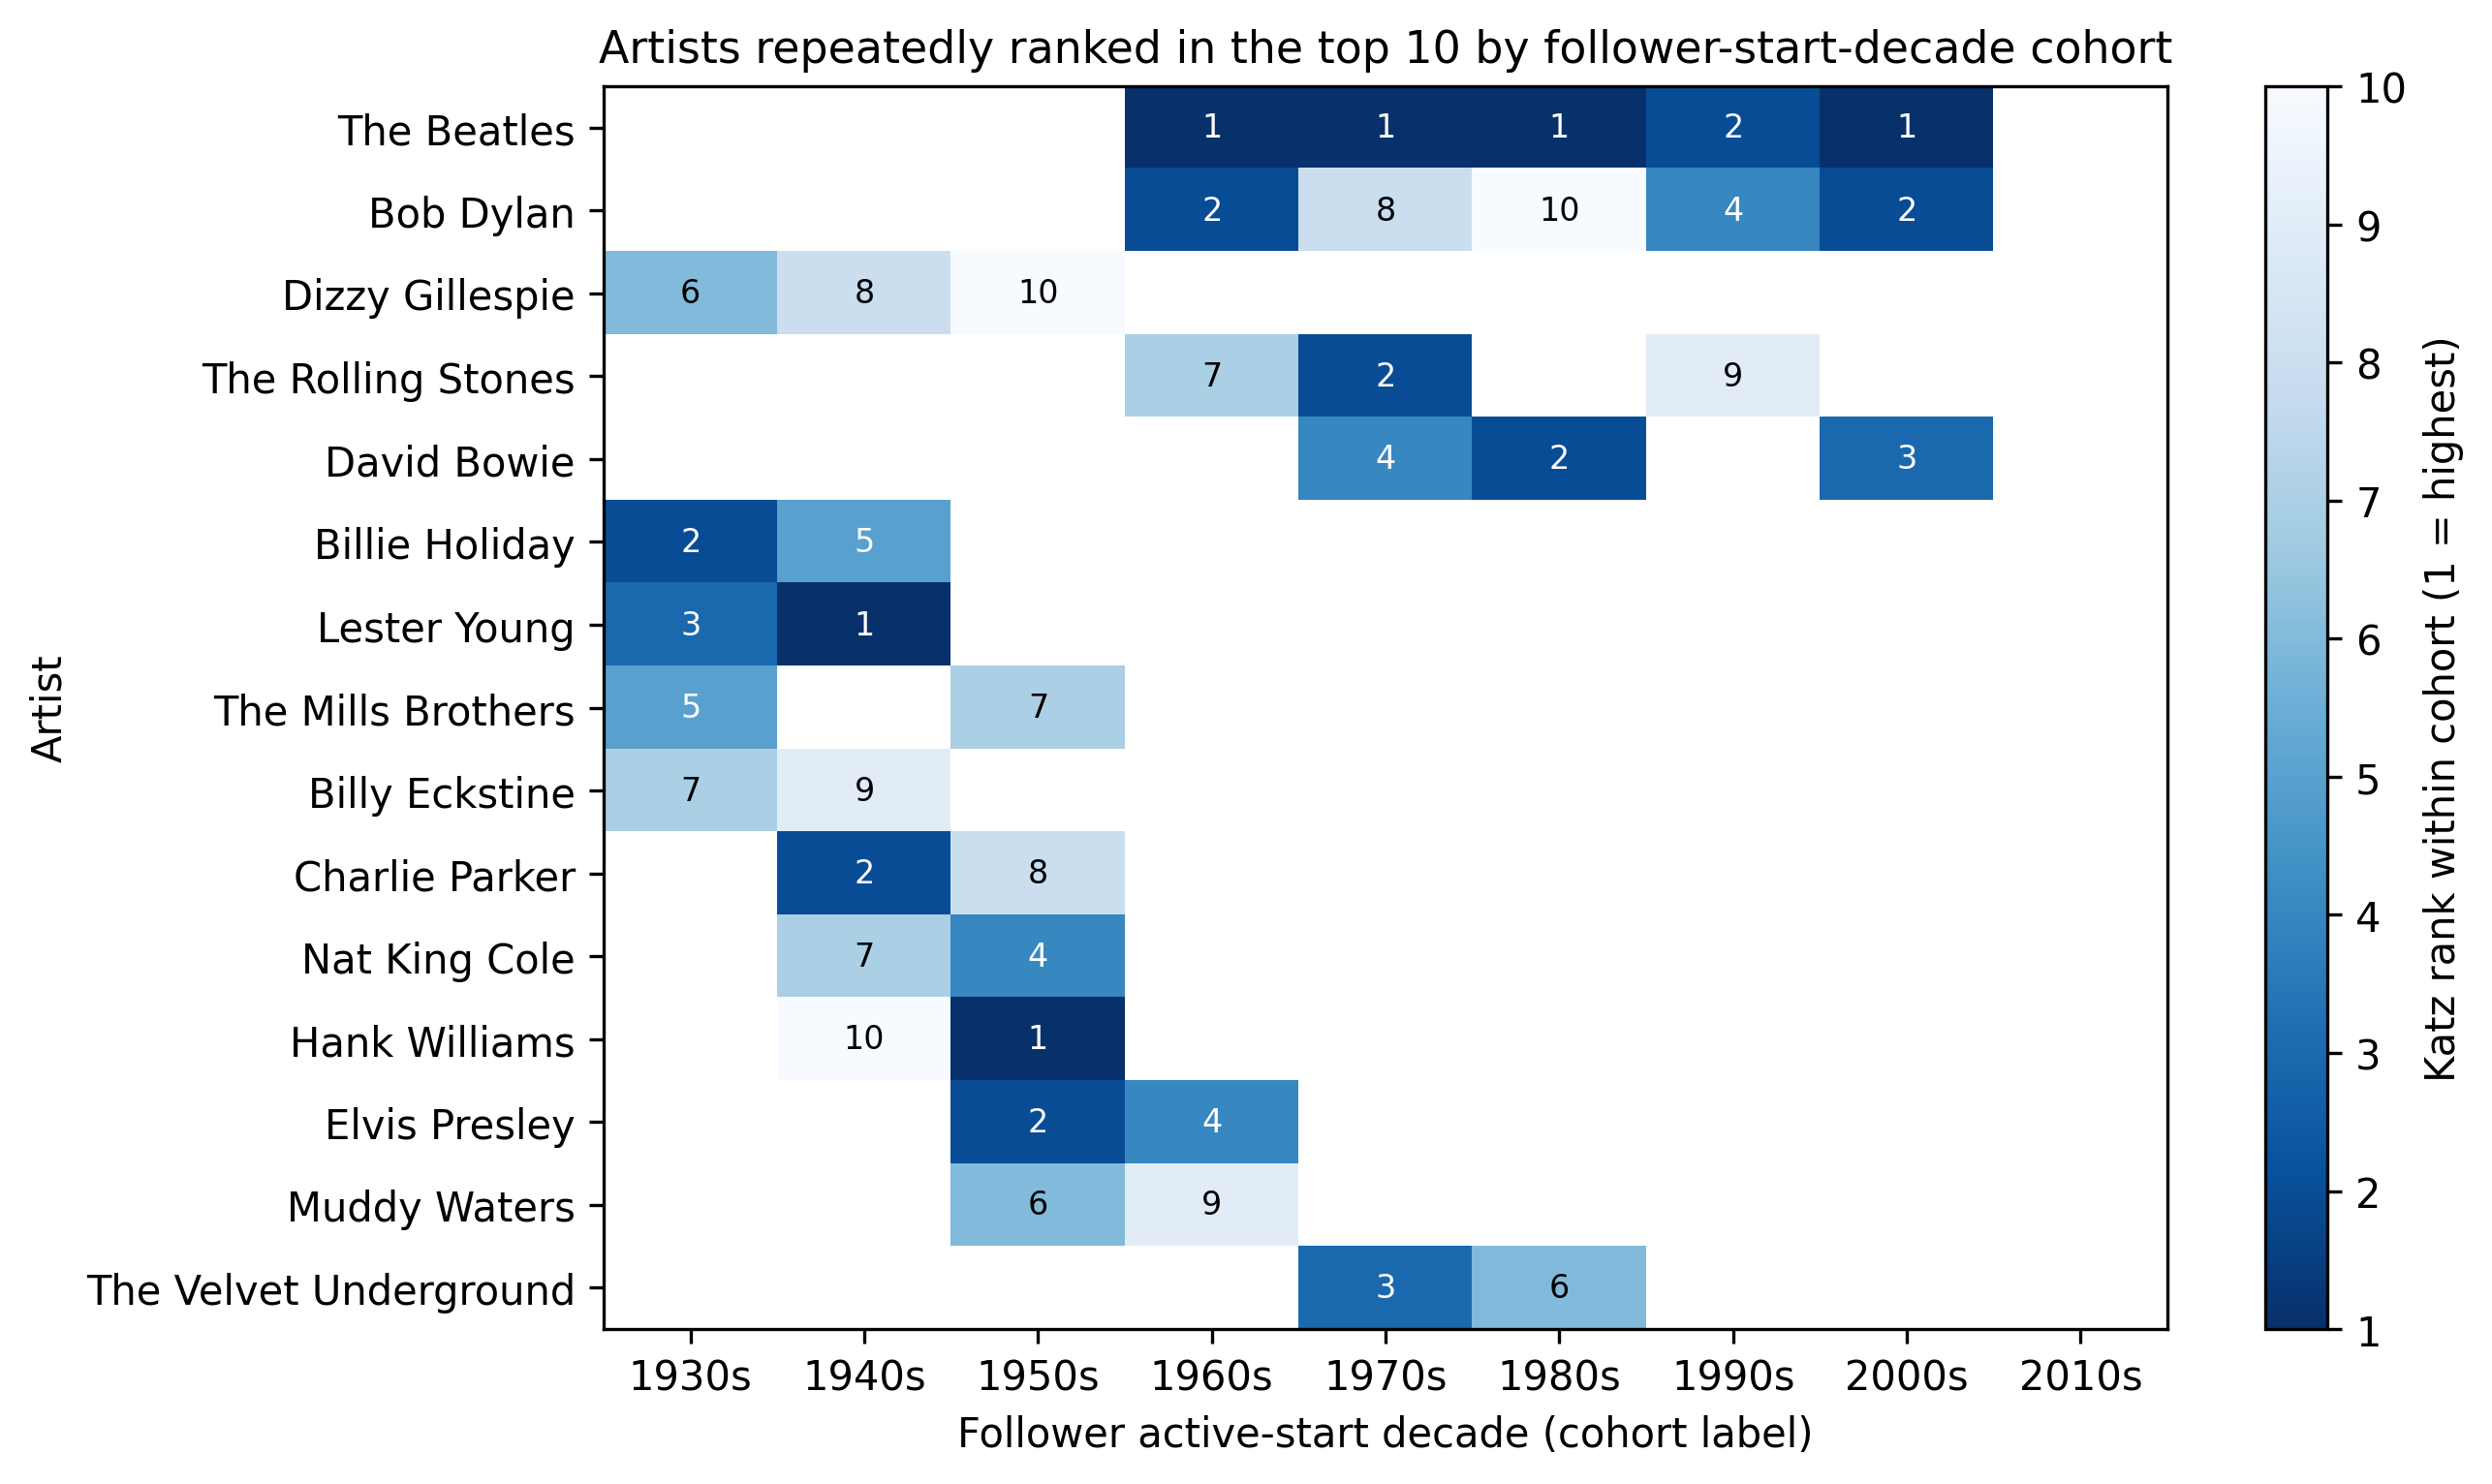
\includegraphics[width=0.92\textwidth]{fig3_cohort_heatmap.png}
\caption{Artists repeatedly ranked in the top 10 within
follower-start-decade cohorts. Each cell gives the artist's Katz rank inside
the cohort of followers who began in that decade (1 = highest; white = not in
the cohort's top 10). Cohorts group by followers' active-start decade, not by
the date an influence occurred; the 2010s cohort is small (811 edges) and its
column is correspondingly sparse.}
\label{fig:q1-cohorts}
\end{figure}

\begin{table}[htbp]
\centering
\caption{Follower-start-decade cohorts: size and three highest-scoring
influencers within each cohort (\(\alpha=0.10\)).}
\label{tab:q1-cohorts}
\begin{tabular}{lrrl}
\toprule
Cohort & Edges & Artists & Top-3 influencers within cohort \\
\midrule
1930s & 193   & 151  & Cab Calloway, Billie Holiday, Lester Young \\
1940s & 741   & 371  & Lester Young, Charlie Parker, Roy Acuff \\
1950s & 2{,}860  & 903  & Hank Williams, Elvis Presley, Ray Charles \\
1960s & 6{,}478  & 1{,}475 & The Beatles, Bob Dylan, Chuck Berry \\
1970s & 6{,}781  & 1{,}878 & The Beatles, The Rolling Stones, The Velvet Underground \\
1980s & 8{,}523  & 2{,}336 & The Beatles, David Bowie, Black Sabbath \\
1990s & 10{,}911 & 2{,}996 & Nirvana, The Beatles, Neil Young \\
2000s & 5{,}472  & 2{,}393 & The Beatles, Bob Dylan, David Bowie \\
2010s & 811   & 690  & Usher, Michael Jackson, Rihanna \\
\bottomrule
\end{tabular}
\end{table}

\subsection{A Genre-Induced Subnetwork: Jazz}\label{subsec:q1-jazz}

Task~1 also asks for a description of a subnetwork; we induce one by
keeping only edges whose \emph{both} endpoints are Jazz, yielding
$G_{\text{Jazz}}$ with 384 artists and 1{,}769 edges (density 0.012),
fragmented into 353 strong components. Jazz is a convenient slice---large
enough to be structurally informative, spanning nine decades, with a
well-documented internal history (swing $\to$ bebop $\to$ cool/hard bop
$\to$ fusion) that gives an external check on the model's ordering. The
leader by within-genre Katz is Charlie Parker (78 direct Jazz followers),
ahead of Lester Young and Miles Davis (83): the depth-over-breadth
mechanism of \cref{subsec:q1-global} recurs inside a single genre, and the
generational reading of \cref{fig:q1-jazz} (swing-era hubs feeding bebop-era
hubs, who feed later artists) mirrors the documented stylistic succession.
The subnetwork also \emph{exports} influence heavily: 409 further edges run
from Jazz artists to Pop/Rock artists, a cross-validation anchor we use in
\cref{subsec:q3-inf-time}. This same subnetwork is revisited in
\cref{sec:model-temporal} as the case study for Task~6.

\begin{figure}[htbp]
\centering
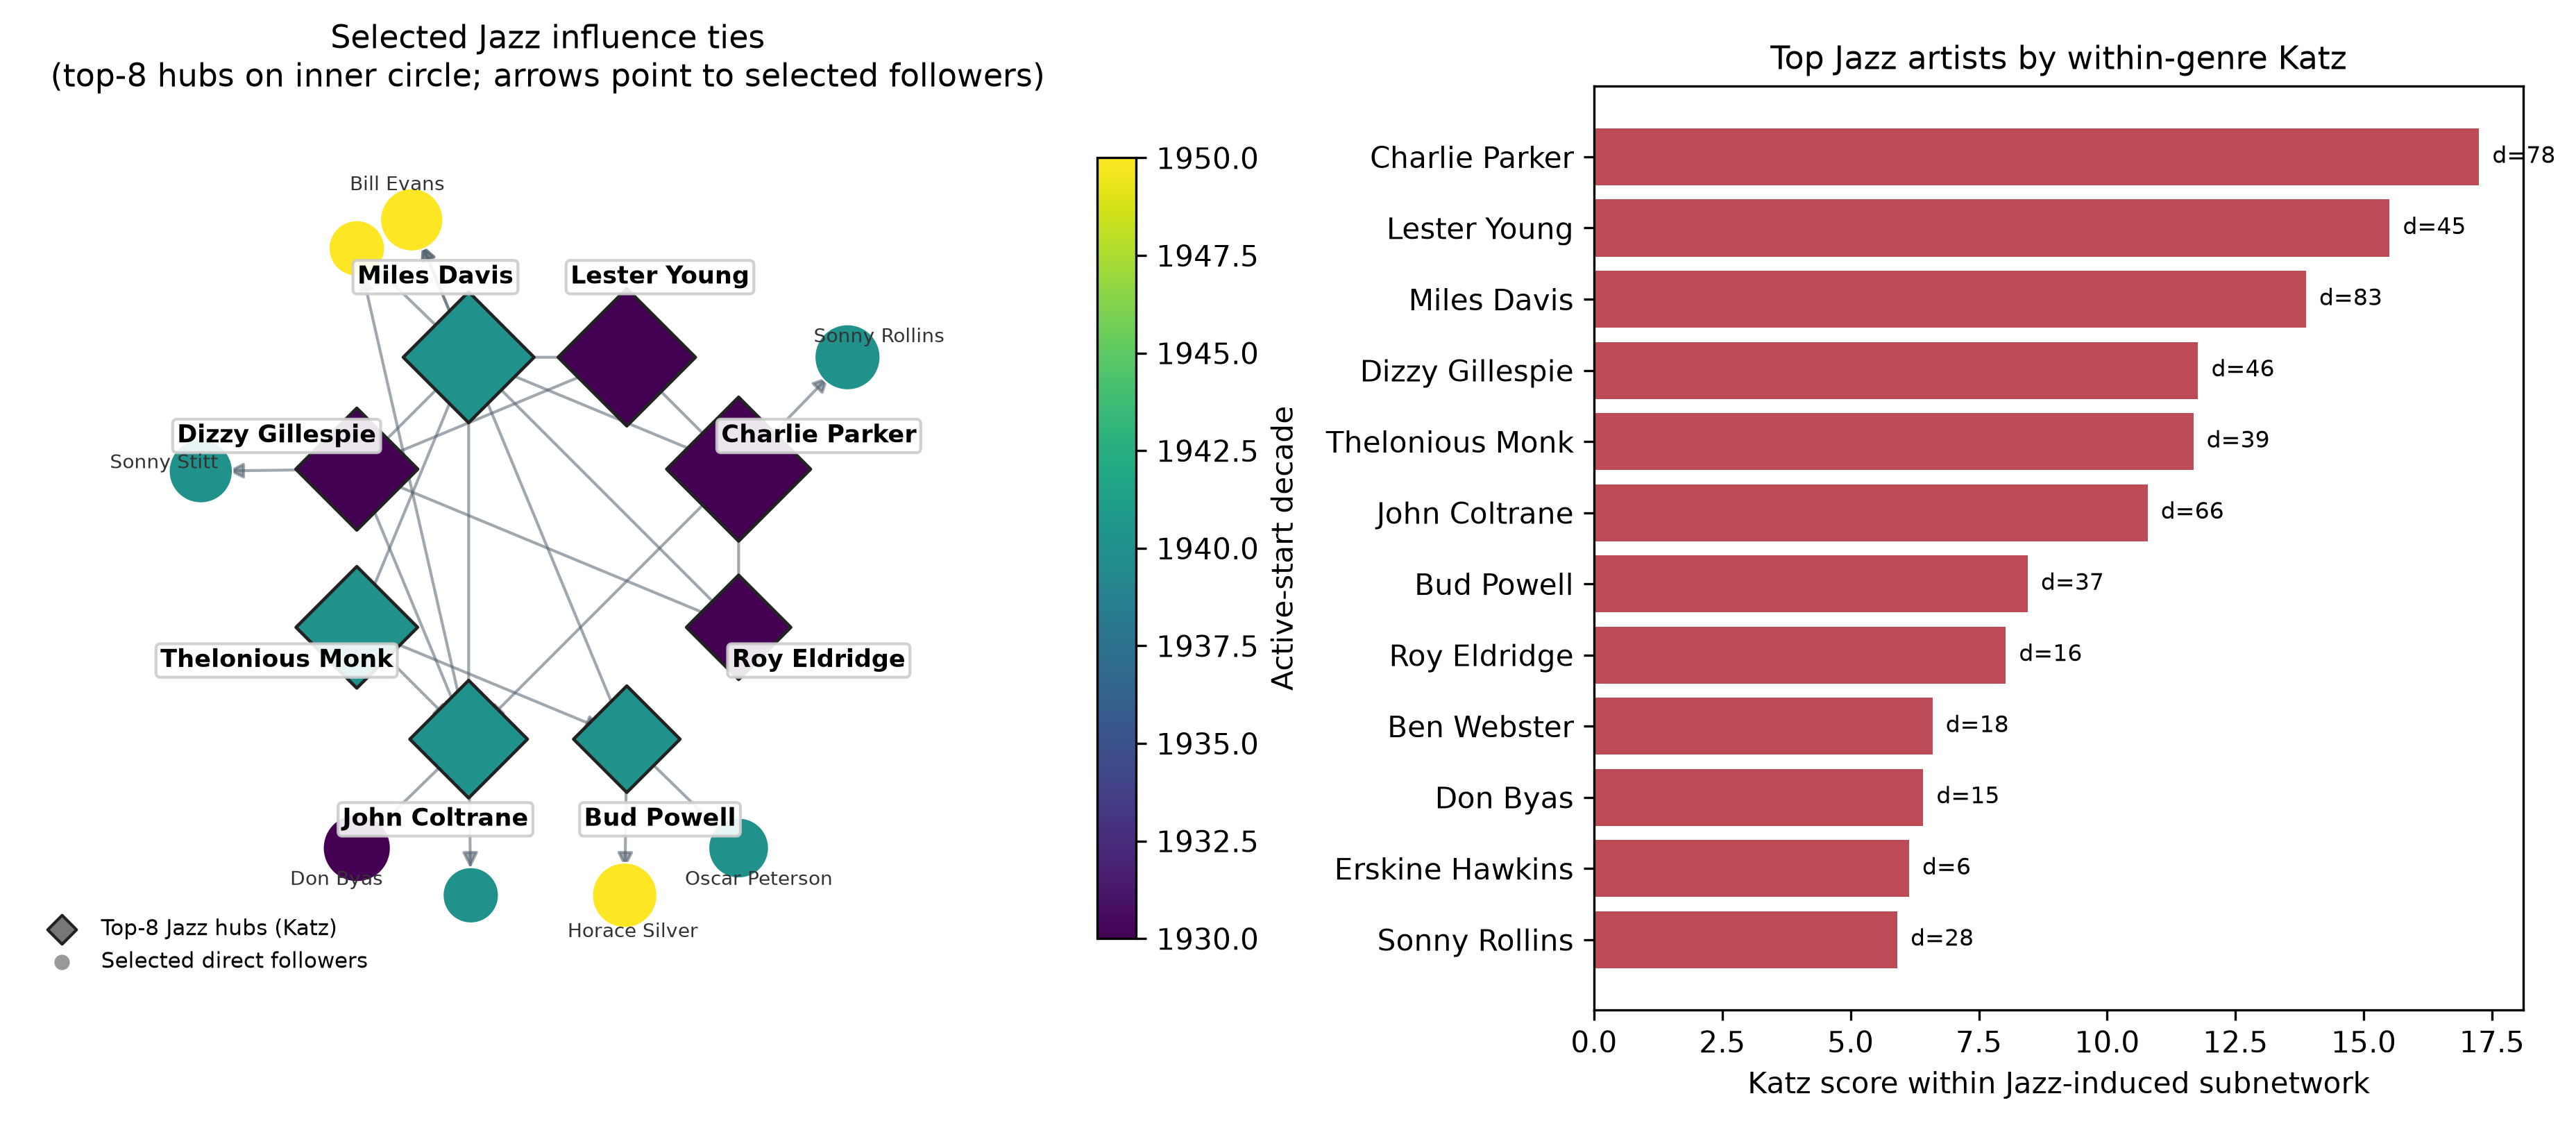
\includegraphics[width=\textwidth]{fig4_jazz_subnetwork.png}
\caption{The Jazz-induced subnetwork. \emph{Left:} selected ego view of the
top-8 Jazz hubs (diamonds, inner circle) and up to three high-scoring direct
followers each (circles, outer rays); arrow direction follows the reported
influence; colour encodes active-start decade and size the within-genre
Katz score. \emph{Right:} top-12 Jazz artists by within-genre outgoing Katz
(\(\alpha=0.10\)); annotations give direct Jazz followers \(d\).}
\label{fig:q1-jazz}
\end{figure}

\subsection{Robustness of the Rankings}\label{subsec:q1-robustness}

\Cref{fig:q1-sensitivity} verifies that the reported rankings do not depend
on analyst choices. \emph{Parameter sensitivity:} recomputing Katz over
\(\alpha\in[0.02,\,0.25]\) (the convergence bound is 0.2767), the bulk
ranking is stable---Spearman correlation with the baseline \(\alpha=0.10\)
never falls below 0.975---and the top-20 overlap is maximised exactly at the
operating point (\(20/20\) at \(\alpha=0.10\); \(16\)--\(20\) for
\(\alpha\in[0.075,0.125]\)), declining toward the extremes of the sweep
(\(9/20\) at \(\alpha=0.02\), \(8/20\) at \(\alpha=0.25\)). The extremes are
semantically degenerate rather than alarming: as \(\alpha\to0\) Katz
collapses toward raw out-degree, and as \(\alpha\) approaches the
convergence bound indirect terms dominate, so divergence there merely
reflects the intended behavioural differences. The choice
\(\alpha=0.10\) sits at the peak of both curves, comfortably inside the
stable interior. \emph{Time-filter sensitivity:} removing all 733
reversed-decade-order edges changes the Katz scores only marginally
(\(\rho=0.986\) against the primary network) and the top-20 sets are
identical (20/20 overlap). We therefore retain all reported edges in the
primary model, as stated in \cref{subsec:net-construction}.

\begin{figure}[htbp]
\centering
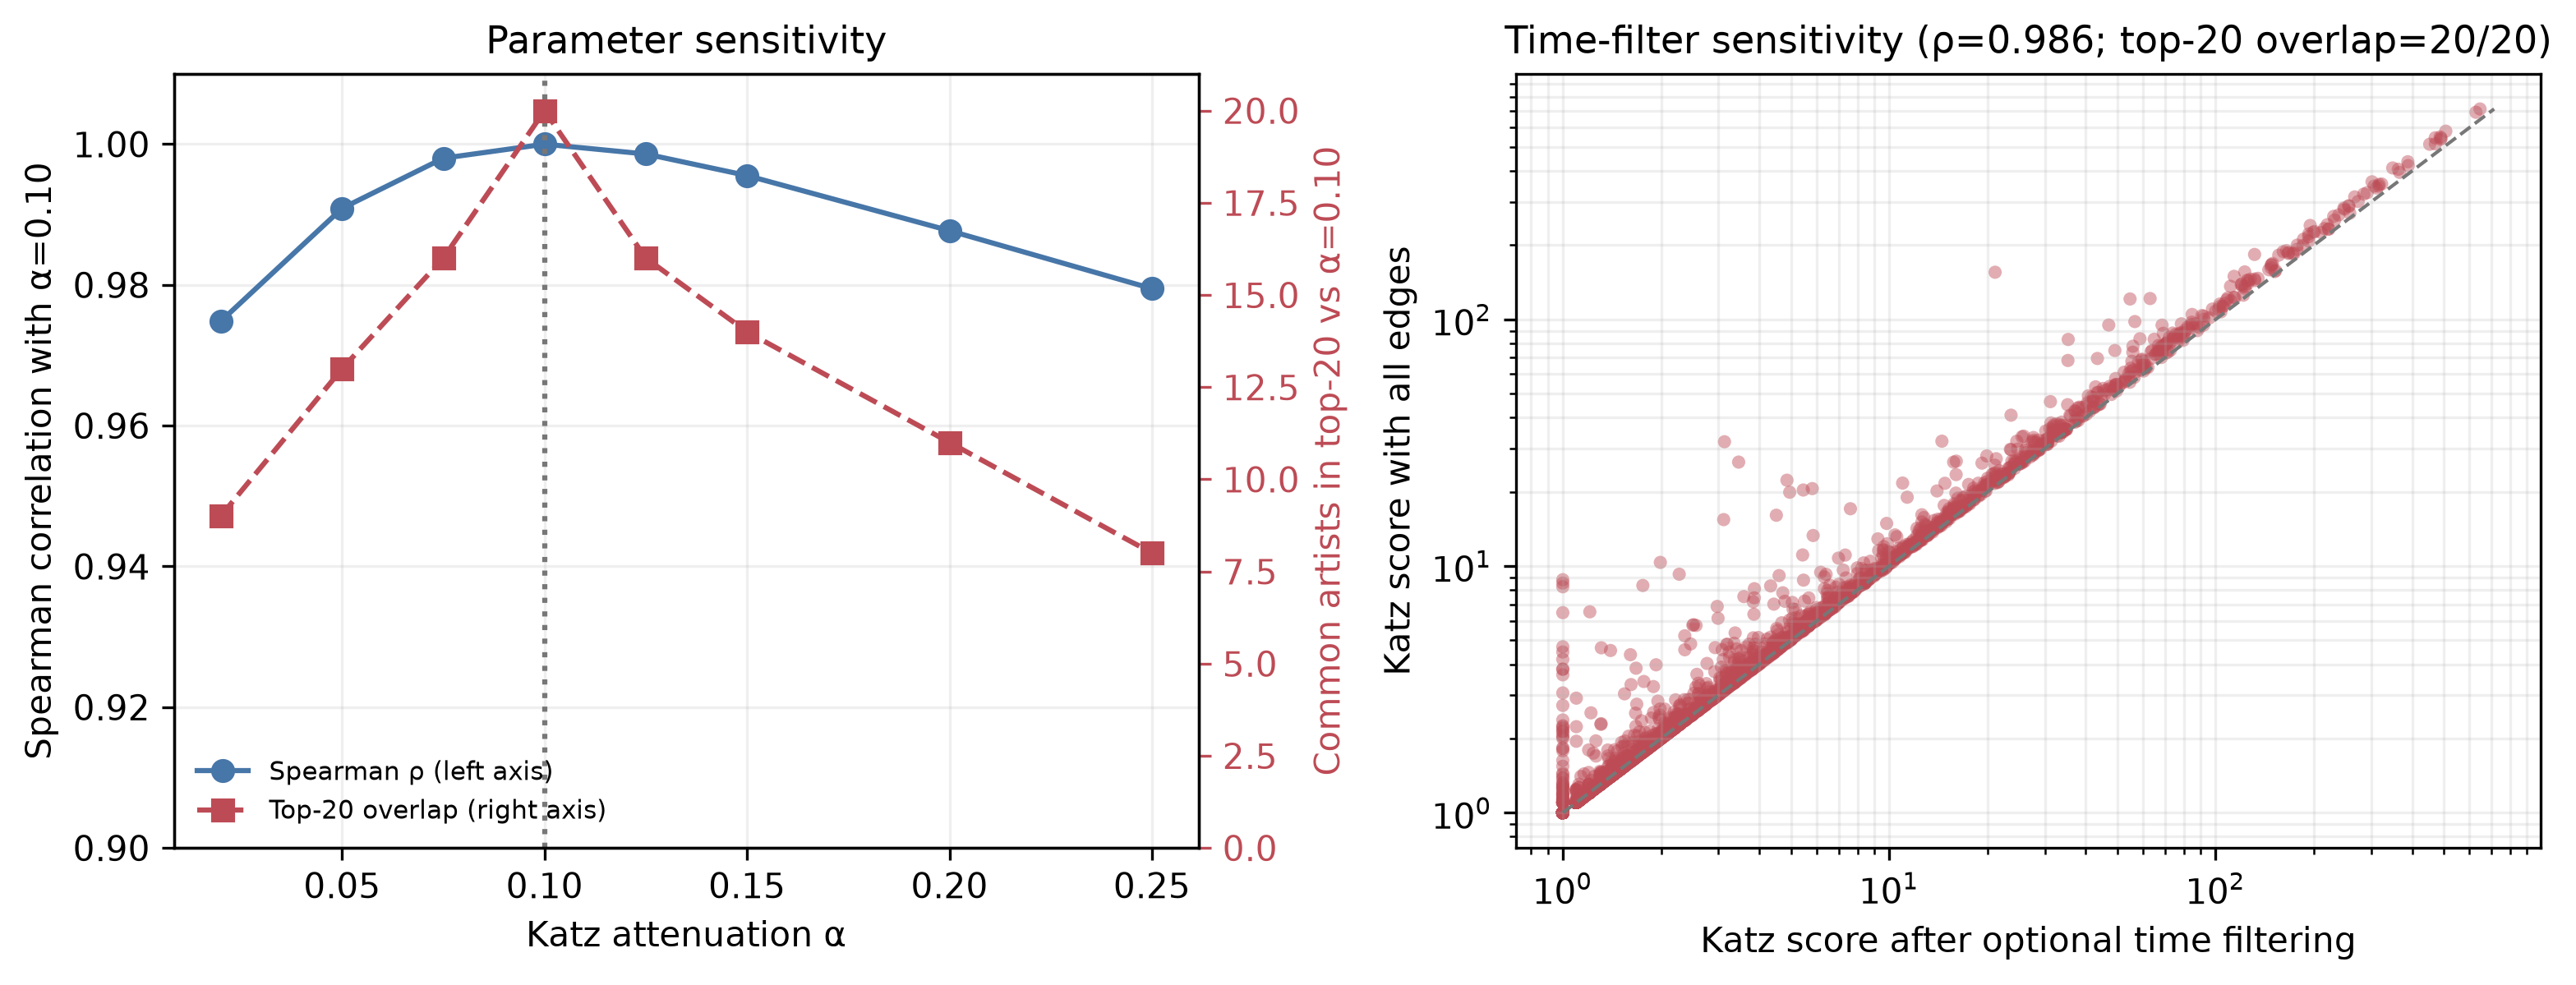
\includegraphics[width=0.95\textwidth]{fig2_sensitivity.png}
\caption{Robustness of the Katz ranking. \emph{Left:} sensitivity to the
attenuation factor: Spearman correlation between the baseline ranking
(\(\alpha=0.10\), dotted line) and rankings recomputed at other levels
(blue, left axis), and the number of artists common to the top-20 of both
rankings (red, right axis); both are maximised at the operating point.
\emph{Right:} per-artist Katz scores with all edges versus scores after
removing the 733 time-order-reversed edges; the dashed line marks equality.}
\label{fig:q1-sensitivity}
\end{figure}

Finally, the three measures corroborate one another in bulk (pairwise
Spearman $\rho$ between 0.95 and 0.97) while their top-20 sets overlap in
only 4--8 of 20 names---high bulk agreement with low top-rank overlap is
precisely the signature of a stable shared backbone topped by artists
specialised for different roles, which supports reporting the measures
separately instead of collapsing them into one index. Across all measures
we emphasise that edges are \emph{reported} relationships, not established
causal influence.


\section{Model II: Measures of Music Similarity}\label{sec:model-similarity}

This section addresses the second requirement of Problem~C: developing a quantitative measure of musical similarity from audio features, and testing whether artists within the same genre are more similar than artists from different genres. We use the existing \texttt{main\_genre} labels in \texttt{influence\_data}; we do not redefine genres such as Pop/Rock.

\subsection{Feature Representation}

For each artist $i$, we form a feature vector $\mathbf{x}_i \in \mathbb{R}^{p}$ from \texttt{data\_by\_artist}, using the Spotify audio attributes
\[
\begin{aligned}
\{\,&\text{danceability},\ \text{energy},\ \text{valence},\ \text{tempo},\ \text{loudness},\\
&\text{acousticness},\ \text{instrumentalness},\ \text{liveness},\ \text{speechiness},\ \text{duration\_ms},\ \text{popularity}\,\}.
\end{aligned}
\]
Genre labels are attached by joining on \texttt{artist\_id} with \texttt{influence\_data}. The within-/between-genre test keeps only artists that have a genre label (here $n=5599$ after dropping missing/Unknown labels).

Because these coordinates have incompatible scales (e.g., tempo versus danceability in $[0,1]$), we apply column-wise $z$-score standardization before any distance computation:
\[
\tilde{x}_{ik} = \frac{x_{ik}-\mu_k}{\sigma_k},\qquad k=1,\dots,p.
\]
All distances below are computed in this standardized space.

\subsection{Baseline Measure: Euclidean Distance}

As the primary similarity model, we measure stylistic discrepancy by Euclidean distance. For artists $i$ and $j$,
\[
d_{ij} = \bigl\|\tilde{\mathbf{x}}_i - \tilde{\mathbf{x}}_j\bigr\|_2 = \sqrt{\sum_{k=1}^{p}(\tilde{x}_{ik}-\tilde{x}_{jk})^2}.
\]
Smaller $d_{ij}$ means greater musical similarity. When a bounded score is useful for visualization, we may use $s_{ij}=1/(1+d_{ij})$; the formal within-/between comparison is performed on distances.

\paragraph{Why Euclidean distance.}
After standardization, Euclidean distance has a clear geometric reading (``closer points sound more alike''), is easy to reproduce in code, and maps directly onto the within-versus-between question. We emphasize that this is a \emph{distance}, not a correlation coefficient.

\subsection{Within-Genre versus Between-Genre Test}

Let $\mathcal{G}(i)$ denote the main genre of artist $i$. Define the average within-genre and between-genre distances
\[
\bar{d}_{\mathrm{within}}
  = \frac{1}{|W|}\sum_{(i,j)\in W} d_{ij},
\qquad
\bar{d}_{\mathrm{between}}
  = \frac{1}{|B|}\sum_{(i,j)\in B} d_{ij},
\]
where $W$ collects same-genre pairs and $B$ collects cross-genre pairs (pairs are randomly subsampled for computational tractability; seed fixed for reproducibility).

\textbf{Hypothesis.} If the feature geometry aligns with the provided genre taxonomy, we expect
\[
\bar{d}_{\mathrm{within}} < \bar{d}_{\mathrm{between}}.
\]
Empirically, under the standardized Euclidean baseline we obtain
\[
\bar{d}_{\mathrm{within}} \approx 3.73
\quad < \quad
\bar{d}_{\mathrm{between}} \approx 4.55.
\]
Thus the inequality holds globally. Large heterogeneous labels such as Pop/Rock may still show weaker within-genre cohesion than smaller, tighter genres.

To visualize genre neighbourhoods, we also compute each genre's centroid in the standardized feature space and plot the pairwise Euclidean distances between centroids (Figure~\ref{fig:heatmap-baseline}). The diagonal is zero by construction; brighter cells indicate nearer genres (e.g., Latin--R\&B, Country--Latin), while Comedy/Spoken is far from most musical genres.

\begin{figure}[t]
  \centering
  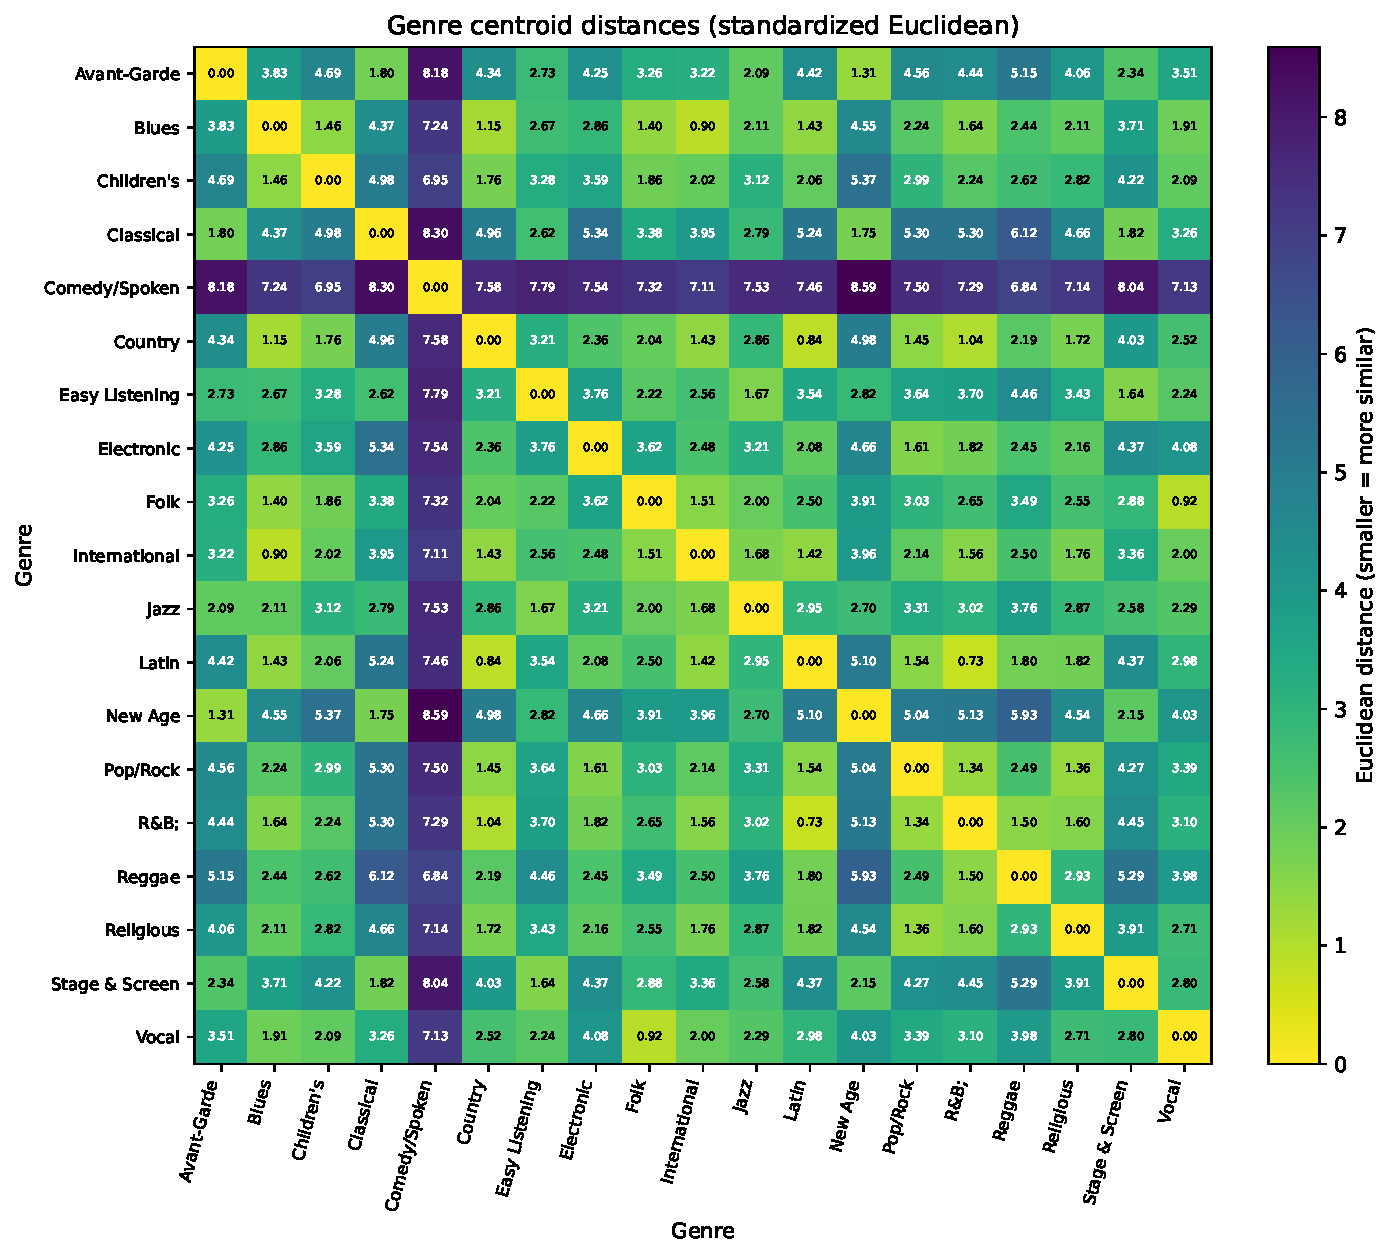
\includegraphics[width=0.62\textwidth]{heatmap_genre_distances_baseline.pdf}
  \caption{Pairwise Euclidean distances between genre centroids in $z$-scored feature space (brighter $=$ more similar).}
  \label{fig:heatmap-baseline}
\end{figure}

\subsection{Robustness Check: PCA then Euclidean Distance}

Audio features are correlated (e.g., energy and loudness), so Euclidean distance in the full standardized space can overweight redundant directions. As a second specification we: (i)~standardize; (ii)~apply PCA retaining enough components to explain at least $80\%$ of variance (here $r=6$, explaining about $82.5\%$); (iii)~recompute Euclidean distances in the score space; (iv)~repeat the within-/between comparison.

Under PCA$\to$Euclidean we again find
\[
\bar{d}_{\mathrm{within}} \approx 3.28
\quad < \quad
\bar{d}_{\mathrm{between}} \approx 4.10,
\]
so the qualitative conclusion is unchanged.

\subsection{Interim Conclusions for Model II}
\begin{itemize}
  \item Musical similarity is operationalized by standardized Euclidean distance on artist-level Spotify features, with PCA$+$Euclidean as a robustness check.
  \item Genres are taken from the dataset; we do not invent new genre definitions.
  \item Both specifications satisfy $\bar{d}_{\mathrm{within}}<\bar{d}_{\mathrm{between}}$.
  \item Similarity is not influence: a small $d_{ij}$ does not imply a declared influence edge (examined later when validating influencers against followers).
\end{itemize}

\section{Model III: Genre Comparison, Distinction and Change}\label{sec:model-genre}

This section addresses the genre-level questions of Problem~C: comparing
similarities (and, with Model~I, influences) within and between genres;
asking what distinguishes a genre; asking how genres change over time; and
asking whether some genres are related to others. Throughout we keep a
single genre representation so that the subsections stay coherent.

\subsection{Genre Representation: Katz-Weighted Feature Centroids}\label{subsec:q3-centroids}

Let \(\tilde{\mathbf{x}}_i\in\mathbb{R}^{p}\) be the globally \(z\)-scored
Spotify feature vector of artist \(i\) (the same \(p=11\) coordinates and
standardization as Model~II), and let \(K_i\) be the outgoing Katz score
from Model~I. For each official main genre \(g\) we define the
\emph{influence-weighted} genre vector
\begin{equation}\label{eq:cg}
\mathbf{c}_g
=\frac{\sum_{i:\,\mathcal{G}(i)=g} K_i\,\tilde{\mathbf{x}}_i}
      {\sum_{i:\,\mathcal{G}(i)=g} K_i}.
\end{equation}
Artists who transmit influence more broadly therefore pull the genre
profile more strongly. An equal-weight centroid is retained only as a
robustness check (off-diagonal correlation of the two distance matrices
\(\approx 0.73\)). After joining Model~II features to Model~I scores we
obtain \(n=5599\) artists across 19 genres.

Between-genre discrepancy is the Euclidean distance
\(d_{gh}=\|\mathbf{c}_g-\mathbf{c}_h\|_2\), with bounded similarity
\(s_{gh}=1/(1+d_{gh})\). Within-genre cohesion is the (Katz-weighted) mean
distance of artists in \(g\) to \(\mathbf{c}_g\). Empirically the mean
within-genre cohesion is \(2.92\), below the mean between-genre centroid
distance \(3.79\): genres remain separated at the aggregate level even
after influence weighting. The closest pairs are Blues--R\&B
(\(d\approx 0.76\)), Blues--Country (\(0.78\)) and Latin--R\&B (\(0.86\));
the farthest involve Avant-Garde against Comedy/Spoken, Children's and
Country (\(d>8\)).

\begin{figure}[t]
\centering
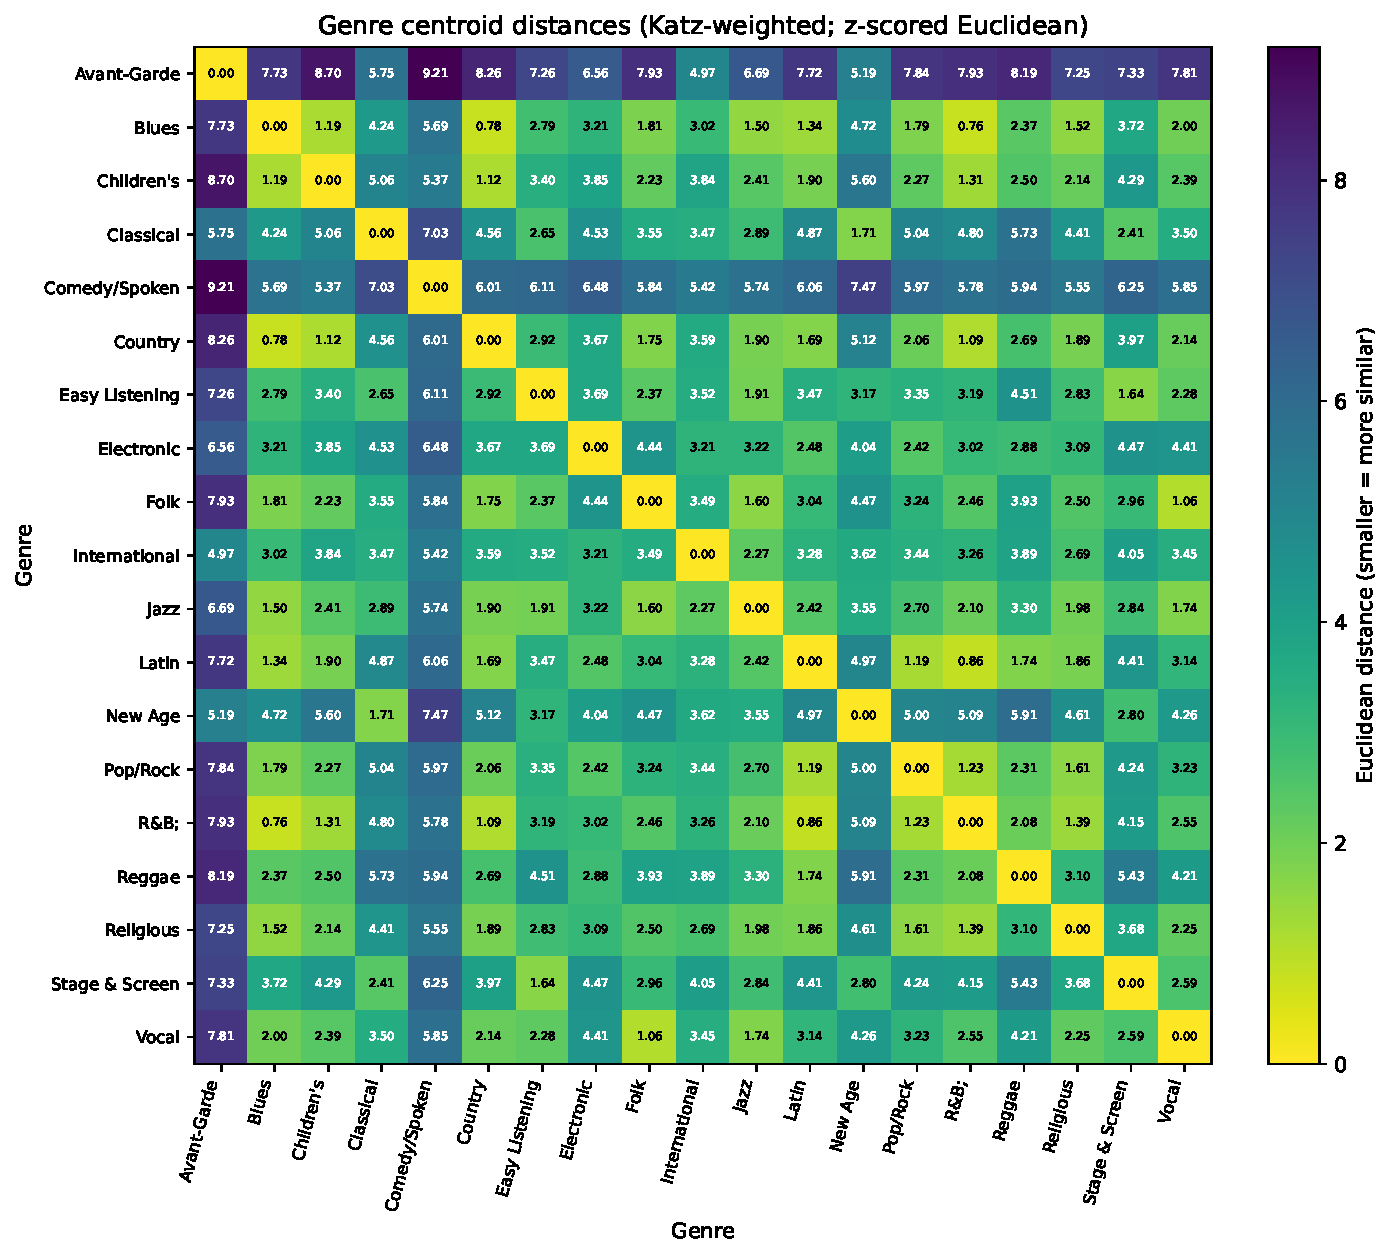
\includegraphics[width=0.65\textwidth]{heatmap_genre_distances_katz.pdf}
\caption{Pairwise Euclidean distances between Katz-weighted genre
centroids \(\mathbf{c}_g\) (smaller $=$ more similar).}
\label{fig:q3-genre-dist}
\end{figure}

\subsection{What Distinguishes a Genre?}\label{subsec:q3-distinguish}

We do \emph{not} assign each genre a unique exclusive feature: with
\(p=11\) features and 19 genres that would be neither feasible nor
meaningful. Instead we read the \emph{same} vectors \(\mathbf{c}_g\). In
\(z\)-space each coordinate of \(\mathbf{c}_g\) is already a signed
deviation from the all-artist mean, so a genre is distinguished by its
\emph{profile}---which coordinates are high or low together.
The most discriminating coordinates globally are
\texttt{duration\_ms}, \texttt{speechiness}, \texttt{instrumentalness}
and \texttt{valence}. Extreme profiles include Avant-Garde (very long
duration), Comedy/Spoken (very high speechiness) and Classical / New~Age
(high instrumentalness and acousticness, low loudness/energy). By
contrast Pop/Rock, Latin and R\&B lie closest to the global mean
(\(\|\mathbf{c}_g\|_2\) small), consistent with coarse, heterogeneous
labels. Even near neighbours remain separable by a few coordinates: e.g.\
Blues versus R\&B differ mainly in loudness, energy and acousticness.

\subsection{How Genre Similarity Changes over Time}\label{subsec:q3-sim-time}

To study change we keep the definition~\eqref{eq:cg} but index it by the
artist's active-start decade \(t\) (Assumption~A2): \(\mathbf{c}_g(t)\) is
formed from artists of genre \(g\) who \emph{began} in decade \(t\), still
weighted by the Model~I Katz score, in the same global \(z\)-space. A
genre enters decade \(t\) only if at least five such artists are present.
We treat 1950--2000 as the main window; the 1930s and especially the
2010s are sparse (only four genres meet the threshold in the 2010s).

\begin{figure}[t]
\centering
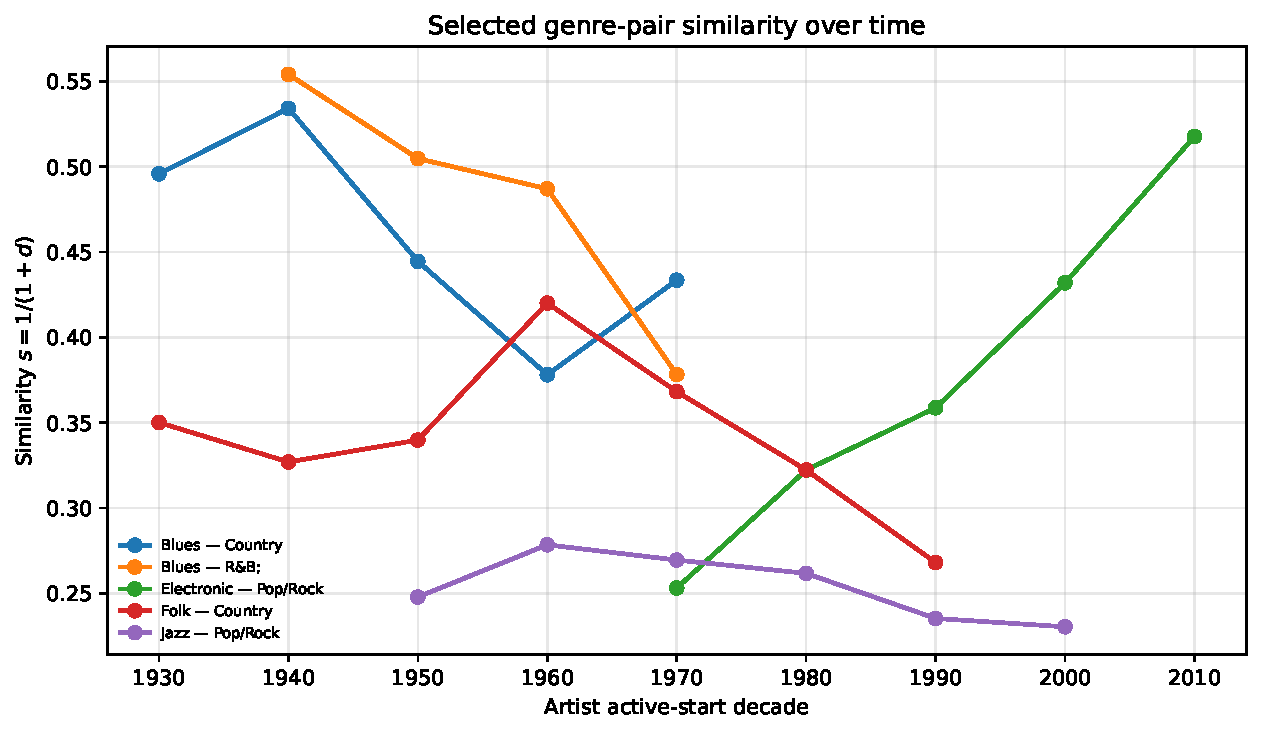
\includegraphics[width=0.65\textwidth]{genre_pair_similarity_over_time.pdf}
\caption{Similarity \(s=1/(1+d)\) for selected genre pairs over decades.
Electronic--Pop/Rock becomes more similar; Blues--R\&B and Folk--Country
trend slightly apart where both are observed.}
\label{fig:q3-pair-time}
\end{figure}

Mean between-genre distance rises from about \(3.16\) (1950s) to about
\(4.55\) (2000s): later cohorts are, on average, more sonically separated.
Pairwise trajectories are heterogeneous---Electronic and Pop/Rock move
closer (\(\Delta s\approx +0.18\) from the 1970s to the 2000s), while
Blues--R\&B similarity falls over the decades in which both are observed.
Self-drift \(\|\mathbf{c}_g(t)-\mathbf{c}_g\|\) is largest for
Comedy/Spoken, International and Classical, indicating that their
decade-specific weighted profiles move farthest from the static
\(\mathbf{c}_g\).

\subsection{How Genre Influence Changes over Time}\label{subsec:q3-inf-time}

% ---------------------------------------------------------------------------
% PLACEHOLDER — teammate (Model I / network side); filled via
% model3_s74_s75_supplement.tex when that file is \input from main.
% ---------------------------------------------------------------------------
\textbf{[Teammate TODO --- genre influence over time.]}
Using the directed network of Model~I, quantify how \emph{influence}
among genres evolves by active-start decade (or edge-endpoint decade):
e.g.\ cross-genre edge counts / share, genre-level outgoing Katz mass, and
export from one genre into another. Place the resulting time series next
to \cref{fig:q3-pair-time} and discuss where sonic similarity and
reported influence move together or diverge.
% End placeholder.

\subsection{Are Some Genres Related to Others?}\label{subsec:q3-related}

% ---------------------------------------------------------------------------
% PLACEHOLDER — synthesize similarity (done) with influence (teammate)
% Can reuse fig:q3-genre-dist and closest/farthest pairs; add a joint
% scatter or two-panel figure: similarity vs cross-genre influence.
% ---------------------------------------------------------------------------
\textbf{[TODO --- relatedness synthesis.]}
The distance matrix in \cref{fig:q3-genre-dist} already supplies a sonic
relatedness graph (Blues--R\&B--Country--Latin as a close cluster;
Avant-Garde as an outlier). Complete this subsection by combining that
picture with Model~I cross-genre influence: genres may be (i)~sonically
close and strongly cross-linked, (ii)~sonically close but weakly linked,
or (iii)~sonically far yet heavily cross-influencing. A short taxonomy of
a few genre pairs under these three regimes answers whether ``related''
should mean sound-alike, citation-linked, or both.
% End placeholder.

\section{Model IV: Temporal Dynamics}\label{sec:model-temporal}

\subsection{Revolutions as Punctuated Leaps (Task~5)}\label{subsec:t5-revolutions}

Task~5 asks which characteristics mark \emph{revolutions} (major leaps) in
musical evolution, and which artists are the corresponding revolutionaries.
We treat change as \emph{punctuated cultural evolution}: variants in a
population drift continuously~\cite{savage2019cultural}, but the rate of
change can spike in short windows~\cite{mauch2015evolution}. Operationally:

\begin{itemize}[leftmargin=1.2em,itemsep=0.2em]
  \item \textbf{Evolution:} gradual movement of the yearly feature state and
  slow change of cross-genre influence shares.
  \item \textbf{Revolution:} a short window in which the sonic leap size is
  anomalous relative to its recent baseline, optionally reinforced by a
  simultaneous restructuring of the influence network.
\end{itemize}

\paragraph{Sonic channel.}
Let \(\mathbf{x}(t)\in\mathbb{R}^{p}\) be the vector of the same \(p=11\)
Spotify features as Model~II, taken from \texttt{data\_by\_year} and
\(z\)-scored across years \(t\in[1930,2010]\). The sonic leap size is
\begin{equation}\label{eq:t5-E}
E(t)=\|\mathbf{x}(t)-\mathbf{x}(t-1)\|_2.
\end{equation}
Because early catalogue aggregates are thin and inflate a global threshold,
we score each \(E(t)\) by a rolling \(z\)-score against the preceding
12 leaps and call a \emph{sonic anomaly} when this local \(z\geq 2\) and
\(t\geq 1948\). The coordinates of \(\Delta\mathbf{x}(t)\) with largest
absolute share identify the driving characteristics of each leap. A Foote-style
past/future window novelty is retained as a robustness companion (same
qualitative peaks).

\paragraph{Network channel.}
We reuse the teammate Model~III flow layer without redefining it: \(F(t)\)
is the genre-to-genre edge count matrix restricted to followers whose
active-start decade is \(t\), with cross-genre share \(c_{\mathrm{cross}}(t)\)
and Katz-weighted share \(c_K(t)\). Decade restructuring is summarised by
\begin{equation}\label{eq:t5-N}
N(t)
=\tfrac12\bigl|\Delta c_{\mathrm{cross}}(t)\bigr|
+\tfrac12\bigl|\Delta c_K(t)\bigr|
+\tfrac14\,\tau(t),
\end{equation}
where \(\tau(t)\) is the \(\ell_1\) turnover of genre shares of outgoing
Katz mass \(K_g(t)\) among artists starting in decade \(t\). Decades with
\(z\)-scored \(N(t)\) above \(0.75\) are network anomalies. This keeps the
same follower-start decade clock as Assumption~A2 and as \(F(t)\), \(c_K(t)\)
in \cref{subsec:q3-inf-time}.

\paragraph{Dual-channel labels.}
A decade is \emph{strong} if it contains at least one sonic anomaly and is a
network anomaly; \emph{weak} if exactly one channel fires; otherwise
\emph{evolution}. Empirically the only strong decade is the 1970s (sonic
peak in 1976; sharp drop in \(c_{\mathrm{cross}}\) and \(c_K\) after the
1950--60s cross-genre high). The 1950s are a network-only weak signal:
\(c_K(t)\) peaks near \(0.53\) while local sonic \(z\) stays below the
cutoff---an influence-structure rewiring (rock \& roll / R\&B export) that
is louder in \(F(t)\) than in yearly mean features. Pre-1948 spikes in raw
\(E(t)\) are plotted but not labelled revolutions (composition caution).

\begin{figure}[t]
\centering
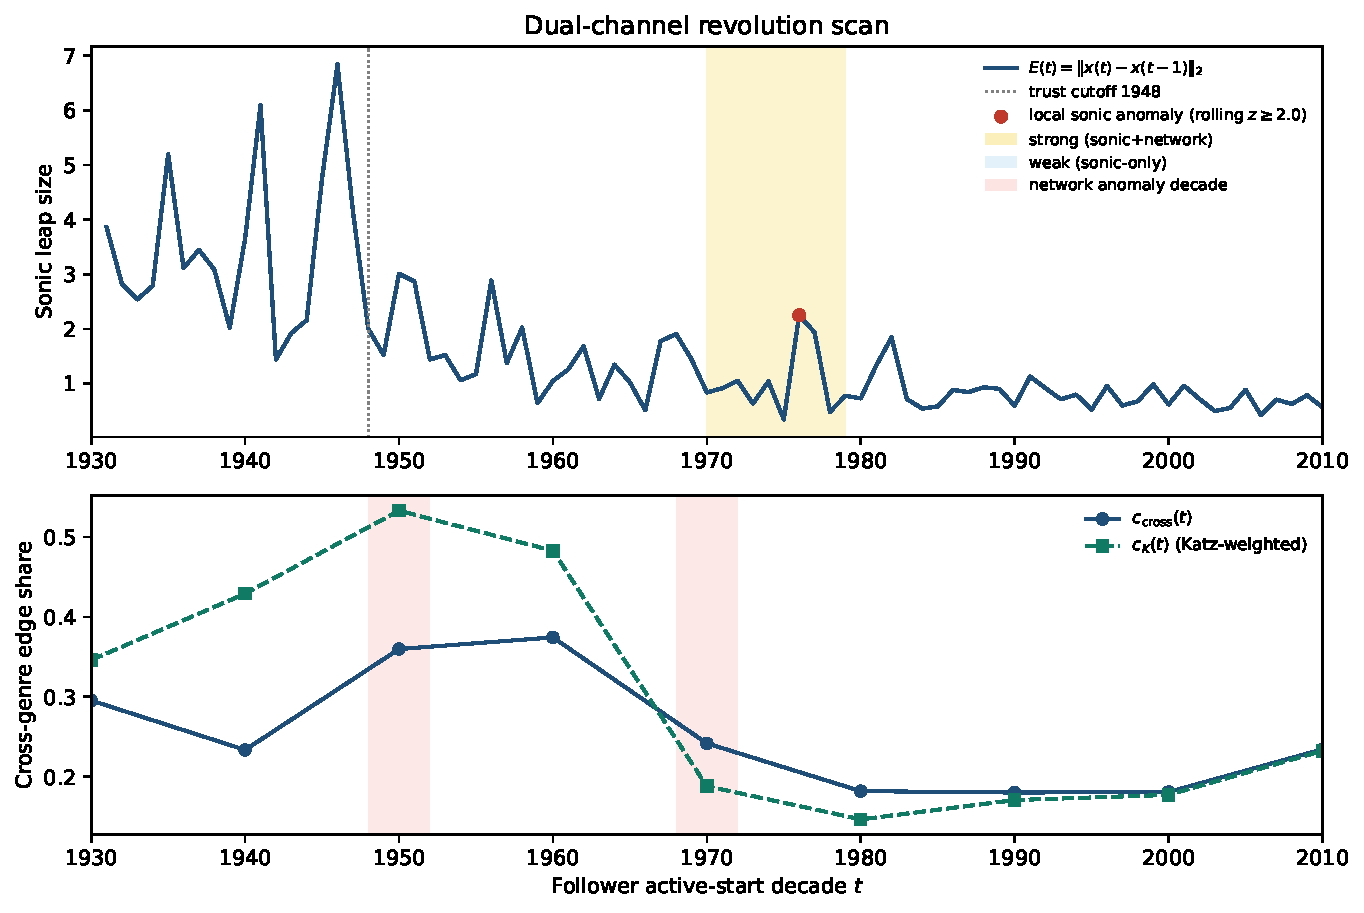
\includegraphics[width=0.68\textwidth]{fig_t5_dual_channel_revolutions.pdf}
\caption{Dual-channel scan: sonic leap \(E(t)\) (top; local \(z\geq 2\),
\(t\geq 1948\)) and network shares \(c_{\mathrm{cross}}(t)\), \(c_K(t)\)
(bottom). Gold = strong 1970s; network-only weak = 1950s.}
\label{fig:t5-dual}
\end{figure}

\paragraph{Characteristics that signify leaps.}
In the strong 1970s window the dominant driver of \(\Delta\mathbf{x}\) is
\texttt{liveness}, followed by \texttt{duration\_ms} and \texttt{tempo}:
the leap is a production/performance shift rather than a single
``genre birth'' coordinate. Network-side, the signifying quantity is the
collapse of cross-genre share after its mid-century plateau
(\(c_{\mathrm{cross}}\approx 0.36\)--\(0.37\) in 1950--60 down to
\(\approx 0.18\) by 1980--2000), i.e.\ influence re-concentrates inside
genres even while sonic drift continues slowly.

\paragraph{Revolutionaries.}
Within a flagged decade \(d\) we score artists who began no later than \(d\)
by a blend of outgoing Katz \(K_i\), the number of followers whose
active-start lies in \(\{d,d+10\}\), and the alignment of their feature
displacement from the previous-decade mean of \(\mathbf{x}(t)\) with the
window's mean sonic direction \(\Delta\mathbf{x}\). This prefers transmitters
who move \emph{with} the leap and are followed afterward, not artists who
merely correlate with the industry average. Top names in the 1950s weak
window include Chuck Berry, Little Richard and James Brown; in the 1970s
strong window, Bob Dylan, The Rolling Stones and Jimi Hendrix
(\cref{tab:t5-revs}).

\begin{table}[htbp]
\centering
\caption{Top revolutionaries by dual-channel window (score blend of \(K_i\),
followers in \(\{d,d+10\}\), and sonic alignment).}
\label{tab:t5-revs}
\small
\begin{tabular}{cllll}
\toprule
Decade & Label & Artist & Genre & \(K_i\) rank signal \\
\midrule
1950s & weak (network) & Chuck Berry & Pop/Rock & high \(K_i\), many 1950/60 followers \\
1950s & weak (network) & Little Richard & Pop/Rock & high alignment + followers \\
1950s & weak (network) & James Brown & R\&B & cross-genre transmitter \\
1970s & strong & Bob Dylan & Pop/Rock & top score in window \\
1970s & strong & The Rolling Stones & Pop/Rock & high \(K_i\) + followers \\
1970s & strong & Jimi Hendrix & Pop/Rock & strong sonic alignment \\
\bottomrule
\end{tabular}
\end{table}

\paragraph{Limits.}
\texttt{data\_by\_year} is a Spotify-era mean catalogue, not a probability
sample of all music; early \(E(t)\) is composition-sensitive. Influence edges
are reported relations, and decade \(t\) indexes follower start years, not
event dates. Detected leaps are statistical rate spikes, offered as
candidates for historical interpretation rather than causal claims.

% T6 is included from main.tex via model4_t6.tex (after this Model IV / Task~5 block).
% TODO (T7): pre/post-1995 era slicing; internet effect on network + features.


\section{Validation and Sensitivity Analysis}\label{sec:validation}
% TODO: validation checks; sensitivity table over key parameters; limitations.

\section{Strengths, Weaknesses and Conclusion}\label{sec:conclusion}
% TODO: strengths; weaknesses; conclusion per task.

%------------------------------------------------------------------------------
% 4. ONE-PAGE DOCUMENT TO THE ICM SOCIETY — must fit on ONE page.
%    Cover: (i) value of our approach; (ii) how richer data would change our
%    work; (iii) recommendations for further study of music and culture.
%------------------------------------------------------------------------------
\newpage
\section*{A Document to the ICM Society}
\addcontentsline{toc}{section}{A Document to the ICM Society}
\label{sec:memo}
\noindent\begin{tabular}{@{}ll@{}}
  \textbf{To:}      & The Integrative Collective Music (ICM) Society \\
  \textbf{From:}    & Team 123090276/123090452/123090773 \\
  \textbf{Subject:} & The value of network-based measures of musical influence \\
  \textbf{Date:}    & November 29, 2026 \\
\end{tabular}
% TODO: memo body (keep within one page).

%------------------------------------------------------------------------------
% 5. REFERENCES — cite every external source of data, ideas, figures and code.
%    Do NOT invent references.
%------------------------------------------------------------------------------
\newpage
\begin{thebibliography}{99}
\bibitem{allmusic} AllMusic. \emph{Music data scraped from AllMusic.com}, 2021.
\bibitem{spotify} Spotify. \emph{Spotify Web API audio features}, 2021.
\bibitem{mauch2015evolution}
  M.~Mauch, R.~M.~MacCallum, M.~Levy and A.~M.~Leroi.
  The evolution of popular music: USA 1960--2010.
  \emph{Royal Society Open Science}, 2(5):150081, 2015.
\bibitem{savage2019cultural}
  P.~E.~Savage.
  Cultural evolution of music.
  \emph{Humanities and Social Sciences Communications}, 5:16, 2019.
\bibitem{katz1953}
  L.~Katz.
  A new status index derived from sociometric analysis.
  \emph{Psychometrika}, 18(1):39--43, 1953.
\end{thebibliography}

%------------------------------------------------------------------------------
% 6. CONTRIBUTION STATEMENT — final page, NOT counted in the 25-page limit.
%------------------------------------------------------------------------------
\newpage
\section*{Contribution Statement}
% TODO: who did what, ordered by ascending student ID; note the code README.
\begin{itemize}
  \item \textbf{Li Peixuan (123090276):} ...
  \item \textbf{Qian Chenghao (123090452):} ...
  \item \textbf{Yu Zihan (123090773):} ...
\end{itemize}

\end{document}
